\chapter{Introduction}

Anthropogenic climate change represents a significant and pressing global challenge, described by the Intergovernmental Panel on Climate Change (IPCC) as ``a threat to human well-being and the health of the planet" \cite{ipcc_2022}. The driving force behind climate change has to do with the emissions of green house gases into the atmosphere. Data from the United States Environmental Protection Agency indicate that carbon dioxide (CO$_2$) accounts for nearly three-quarters of those greenhouse emissions \cite{epa_2019}. 
%A breakdown of emissions by sector can be seen in figure \ref{fig:green_house_gas_emissions}.

\begin{figure}[h!]
	\centering
	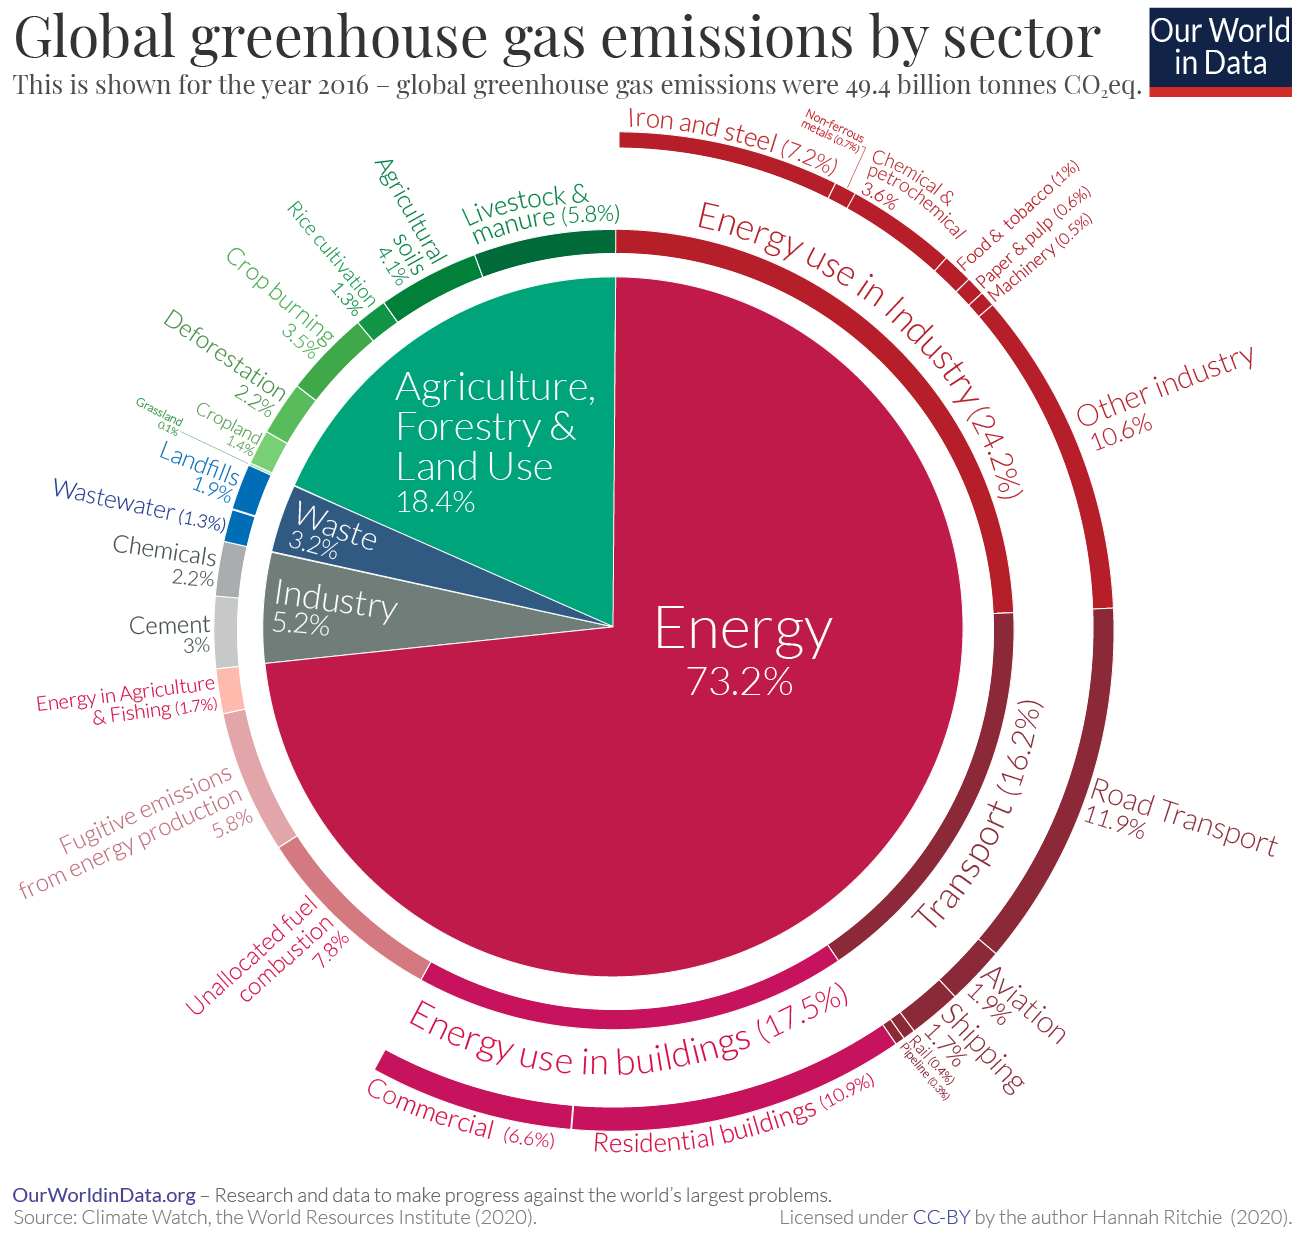
\includegraphics[width=\linewidth]{chapter_1/figures/emissions.png}
	\caption{Global greenhouse gas emissions by sector for the year 2016 \cite{ritchie_roser_2020}.}
	\label{fig:green_house_gas_emissions}
\end{figure} 

As seen in figure \ref{fig:green_house_gas_emissions}, global greenhouse emissions originate from a diverse array of sources and processes. Hence, concentrating mitigation efforts exclusively within certain sectors, such as transport or electricity generation, are insufficient. While the current progress of reducing humanities reliance on fossil fuels through the adoption of renewable energy sources and the transition to electric vehicles is an important step forward, achieving the mark of net-zero emissions necessitate innovations across various other sectors. At present, there is no one solution to climate change.

One promising technology for addressing residual emissions and progressing toward net-zero targets is carbon capture and storage (CCS). It should be stressed that CCS alone cannot fully solve the climate crisis, instead it should be viewed as an indispensable component in a broad and comprehensive strategy to achieve net-zero emissions. 

CCS represents a suite of  processes that focus on either preventing the release of CO$_2$ into the environment or removing existing CO$_2$ in the atmosphere. The captured CO$_2$ would first be compressed, then transported for storage. The CO$_2$ storage typically entails injecting the gas into deep underground rock formations which essentially function as a geological reservoir \cite{IEA2020}.

The quintessential application of CCS lies in sectors that are otherwise challenging to decarbonise, such as the manufacturing of cement. Here, the CO$_2$ released stems from the chemical process, i.e. the conversion of calcium carbonate (CaCO$_3$) to calcium oxide (CaO), rather than through combustion. While the ambitions to implement CCS in this sector has been slow, in 2025 Norway is set to bring the world’s first cement factory with CCS online \cite{brevikccs2024mechanical}. 

The other approach to CCS would be using direct air capture (DAC) technologies, which extract the CO$_2$ from the ambient air in one of two methods. Solvent-based approaches trap the CO$_2$ in a liquid chemical, then rely on heating to release the CO$_2$ gas \cite{An2023}. Sorbent-based approaches use solid filters that bind with the CO$_2$, then with the use of low pressure, the desorption CO$_2$ molecules from the filters can occur \cite{An2023}. Nonetheless, because the CO$_2$ concentration in the air is proportionally tiny, DAC should preferably be used as one of the methods to address legacy emissions already accumulated in the atmosphere.

While conventional CCS methods primarily focus on the sequestration of CO$_2$ for long-term storage, the captured of CO$_2$ itself can serve as a valuable feedstock for industrial applications. This is known as carbon capture and utilisation (CCU), and aims to recycle CO$_2$ into useful chemical products for industry. Several viable pathways exist for CO$_2$ utilisation, including thermal decomposition, electro-catalysis, and with the use plasmas \cite{Khunda2023}. However, each of these approaches presents distinct challenges.

Thermal decomposition requires high temperatures, leading to significant energy consumption and reduced overall efficiency. Similarly, electro-catalytic conversion typically relies on noble metal catalysts which can be quite expensive and are often times not environmentally friendly \cite{Khunda2023}. In contrast, plasma-assisted CO$_2$ conversion - also referred to as plasma-assisted CO$_2$ splitting - has emerged as a promising method, as it operates at low temperatures and atmospheric pressures, without the need for catalysts. 

To generate and sustain the plasma, inert feed gases (typically argon or helium) are commonly employed due to their chemical non-reactivity. This inert behaviour minimises the likelihood of unwanted  reactions with co-reactants, which would be CO$_2$ in this context. Furthermore, CO$_2$ is known as a molecular gas (similar to nitrogen and oxygen), thus possess vibrational and rotational energy levels. As a result, it can absorb and dissipate energy to heat loss, rather than sustaining the ionisation of the plasma. In comparison, inert gases lack these energy levels, reducing energy dissipation via quenching and allowing the plasma to be sustained for longer durations.

However, the major drawback of using inert gases is their high cost. Current CO$_2$ conversion techniques often involve venting waste gases (including both the inert gas and unconverted CO$_2$) directly into the atmosphere. While this approach is feasible in a laboratory setting, its economic viability becomes increasingly untenable at an industrial scale. As such this research aims to investigate the feasibility of recycling the vented gases, which would should drastically improve the cost savings associated with this carbon utilisation technique. 

With that in mind, the remainder of this report is structured as follows. Chapter 2 introduces the concept of plasma discharges, outlining the fundamental principles and some examples of discharge sources. Chapter 3 provides an overview of the CO$_2$ splitting process, presenting the relevant background information and detailing the particular process chosen for this research. Chapter 4 describes the design and manufacturing of the plasma discharge source used, including some preliminary tests with the feed gas and CO$_2$. Chapter 5 presents the engineering and development of the closed system designed for the recycling of gases. Chapter 6 describes the plasma reactor design utilised to facilitate organic synthesis from the CO$_2$ splitting process. Finally, the conclusion summarises the key findings of this research, discusses the implications, and elaborates on the future work required to scale this process to industrial applications. 



\section{Contribution to knowledge}

TODO: Once finalised the conclusion